\title{What does it take to create with domain-appropriate tools?}
\subtitle{A case study on the ``OROM'' system}
\author{Joel Jakubovic}
\affiliation{University of Kent, Canterbury}

\maketitle

\newcommand{\joel}[1]{}
\newcommand{\svgel}[1]{\texttt{\textless{}#1\textgreater{}}}
\newcommand{\OSFA}{One-Size-Fits-All}

\begin{abstract}
There is a One-Size-Fits-Allquality to languages, APIs and even programming itself. Whether you're making a mobile game or a scientific simulation, you will be using a text-based language with similar devices for structuring your code. This is a source of artificial difficulty in creating, understanding, and modifying software systems. No matter the domain, the author's design needs encoding into a form that does not resemble it.

This paper describes a vision where software can be built in a programming environment that is closer to the domain of the software itself. By doing so, users of the system can use familiar abstractions and tools for adapting it. A step towards this vision is presented: a Web version of a minimal OOP system, developed as an executable version of the diagrams of its design, in a substrate meant to facilitate this. The experience of creating such a substrate is analysed, and I suggest deficiencies in programming environments that stand in the way of making this practice commonplace, as well as ways to fill in these gaps.
\end{abstract}

\keywords{substrate, visual, context, domain, adaptation}

\hypertarget{introduction}{%
\section{Introduction}\label{introduction}}

As someone who can code, I have already passed the first and most
important hurdle for making full use of the potential of my computer.
However, even in this supposedly empowered state, I am still far away
from feeling the relationship between myself and software as between
artisan and material, free to shape it into any form with effort
proportional to complexity.

One would have thought that software-creation acts like hypothetical
super-intelligent AI. That is: even though we start from a primitive
base in the 50s (or even today), there would surely be a recursive
process of self-improvement, building better software-creation tools
with the existing ones, until an ``expressivity singularity'' where
software becomes a workable material as described.

However, this didn't happen. Or at least, it is happening glacially
slowly. The brute fact is that whenever you want to create software, you
go to a text editor and figure out how to translate your design into
that. The text editors, being software, were written with the help of
previous text editors, and so on. It's undeniable that text editors have
improved, even if you think it peaked with Emacs. We just don't seem
able to go beyond them where it matters, such as visual domains
ill-fitted to monospaced ASCII.

Amdahl's Law generalises the following idea: even when you spend hours
of effort doubling the performance of a component used 1\% of the time,
your reward is a system overall improved by a mere 0.5\%. Now, text
coding is certainly ubiquitous, the 99\% case in programming, so you
might wonder where I'm going with this. Well, a small improvement to
text editing, if adopted by everyone, certainly does have a massive
\emph{intermediate} effect --- but this only \emph{matters} to the
extent that text was helping the programmers in the first place. If my
goal is to draw or animate pictures, or create a digital synth from a
frequency spectrogram, then giving me the ability to auto-indent my SVG
markup is rather underwhelming as a productivity increase, as it doesn't
target the core of the enterprise that makes it so hard.

My experience of coding, most of the projects requiring shapes (such as
GUIs), leads me to conclude that no matter how much I improve my skill
at a particular language, knowledge of libraries or even general coding
ability, my predicament stays the same. Our basic method of creating
software is optimised for an ever-diminishing proportion of the software
we actually want to make; ill-optimised for the graphics, layout,
interactivity and and basic physics --- more on this later --- that we
usually require.

Whenever I work on these I feel stuck in a box I know I can never escape
from: that box is the text editor, a fixed conduit through which all
\emph{fundamental} changes to my program must pass. It's not a part of
the system I am building, so I can't even make use of features of the
thing I'm developing, to make its own development easier.

Surely the trick is to \emph{use} coding to build something \emph{better
than it}. And then use that, to build something even better. But there
is an enormous breadth and depth of philosophies here, along with many
failed historical attempts to do better --- or at least, ones that
failed to catch on. But even worse than this is that in my very
\emph{language} here I am making the same mistake as the text editor ---
speaking in unqualified terms of ``better'' and ``worse'' as if there
really is a One-Size-Fits-Allsolution to software creation!

Of course what we \emph{really} want is the ability for people to create
\emph{in the way that they think is best} in their particular context
--- to equip them to feasibly create the tools that suit them for the
thing they want to make. And second-order tools that suit them for
making the first-order tools, etc. It would do no good to replace
text-imperialism with anything-else-imperialism, which is one
interpretation of calls for alternatives.

This dream goes beyond the familiar sense of what constitutes a
``craft'', as far as a strong melding of tool and material. Parallels
can be drawn with industrialisation and a strong division of labour: the
community as a whole produces its higher-order tools, but currently no
single person can have the same autonomy. A (future) software craft
could be expected to give this power to \emph{individuals}, instead of
the community alone. Whenever there are many small specialities
(e.g.~languages, tools, or subject areas) each serving many clients, the
One-Size-Fits-Allstyle is the best one can hope for. Adaptation to
individual preferences and idiosyncrasies is only feasible when those
individuals can do it themselves.

What we need is some system that not only lets us create software in a
way that is ``close to the problem domain'' as decided by the
user-developer, but also can augment or change itself to adapt to a
different ``way of creating''. Existing systems seem to only have one of
these properties without the other: Smalltalk and LISP try to minimise
arbitrary commitments of language \emph{semantics} to this end, but
their being textual languages is a fairly tough commitment to break out
of. And it is not so hard to make a specific, \emph{hard-baked} visual
or alternative programming tool --- but it is hard to make it
re-programmable \emph{without} having to go back to \emph{its} textual
source code.

If someone wants to type out pictures in ASCII, let them --- whether
they do it for a challenge, or even if they find that more natural for
themselves. But equally, if I want to do it another way, then please
give me that affordance. This is how I segue into the software artefact
for which I have been attempting to build a natural representation.
True, it is a programmer's artefact, but it is still representative of
what any normal person has to do, insofar as:

\begin{enumerate}
\def\labelenumi{\alph{enumi})}
\tightlist
\item
  Wanting to create a piece of software (for whatever reason)
\item
  Having in mind a natural way to represent it as it's being built.
\end{enumerate}

\hypertarget{the-orom-system}{%
\section{The OROM system}\label{the-orom-system}}

When I first read the paper Open, Reusable Object Models, I was hooked
on its idea of a small but expressive starting system that could be
self-improved into anything. It describes a late-bound\footnote{Fewer
  commitments; more things determined by runtime conditions},
Smalltalk-style\footnote{OOP with more emphasis on object instances and
  messaging (methods) as in a distributed system; less emphasis on class
  hierarchies implementing traditional data structures} objects and
messaging environment that the authors call ``Id'' --- but which I refer
to as OROM, for pronunciation and Googleability.

Essentially, an OROM object is a block of state which can change as a
result of messages received by it. A message is sent by first
\emph{bind}-ing its name to its \emph{implementation}: specific code,
which is then run in the context of the receiver. ``Bind'' is
accomplished via another message send, this time to the receiver's
\emph{vtable}, or ``behaviour''. This is another object whose state
defines a particular way of associating ``message name'' to
``implementation code''. This continues up the vtable-chain, and
terminates at a base case. The system as a whole is ``bootstrapped''
into existence by its initialisation code. Each step of this code makes
use of any parts of the system set up by the previous steps.

The paper itself consists of mostly prose, several code listings, and
full C sources for a sample implementation at the end. It also provides
several diagrams. But to understand it, I repeatedly found myself
drawing \emph{extra} diagrams. For example, the first acts of the
running system boil down to initialising the three or so objects. This
consists of allocating memory, interpreting it as a C struct and then
filling in fields in a mundane manner. I had great difficulty following
the specifics in my head, but when I drew tables in the style of their
diagrams I readily saw what what going on. I personally would have
preferred these to have been in the paper in the first place, but I am
not necessarily representative of those who read it. The
One-Size-Fits-Allapproach is perhaps unavoidable for static media like
print.

Other areas like messaging semantics could still be quite confusing.
After all, should we expect to be able to predict the entire future
evolution of a dynamical system from a static description of its initial
state, such as source code? Is this not why debuggers exist? Having
``de-compiled'' English text and C source code into object diagrams, it
is a shame to have to compile it all back to struct member assignments.

Worst of all, the reference system does not even have text I/O when it
is run, let alone some sort of GUI. That is, the (un)intended user
interface for this project is a C debugger! Faced with the necessity of
adding \emph{some} UI, it seemed a waste of effort to end up with a
system that must be continually polled for its current state at a
terminal prompt. If I naturally think of this system as 2D tables, why
can't that be how the running system looks? I do not have to keep
polling my eyes for what state my diagrams are in.

But further than that --- why can't the system be \emph{built} out of
tables in the first place? Shouldn't this be the main takeaway from the
amount of time we spend prototyping, explaining and designing software
as diagrams on paper? Why must the ``natural representation'' be
restricted to the finished product?

Thus was my natural representation decided. My first attempt to make it
a reality was a partial success: a webpage made of HTML tables, evolved
via JavaScript.

\hypertarget{orom-as-html-tables}{%
\subsection{OROM as HTML tables}\label{orom-as-html-tables}}

\begin{figure}[h]
  \centering
  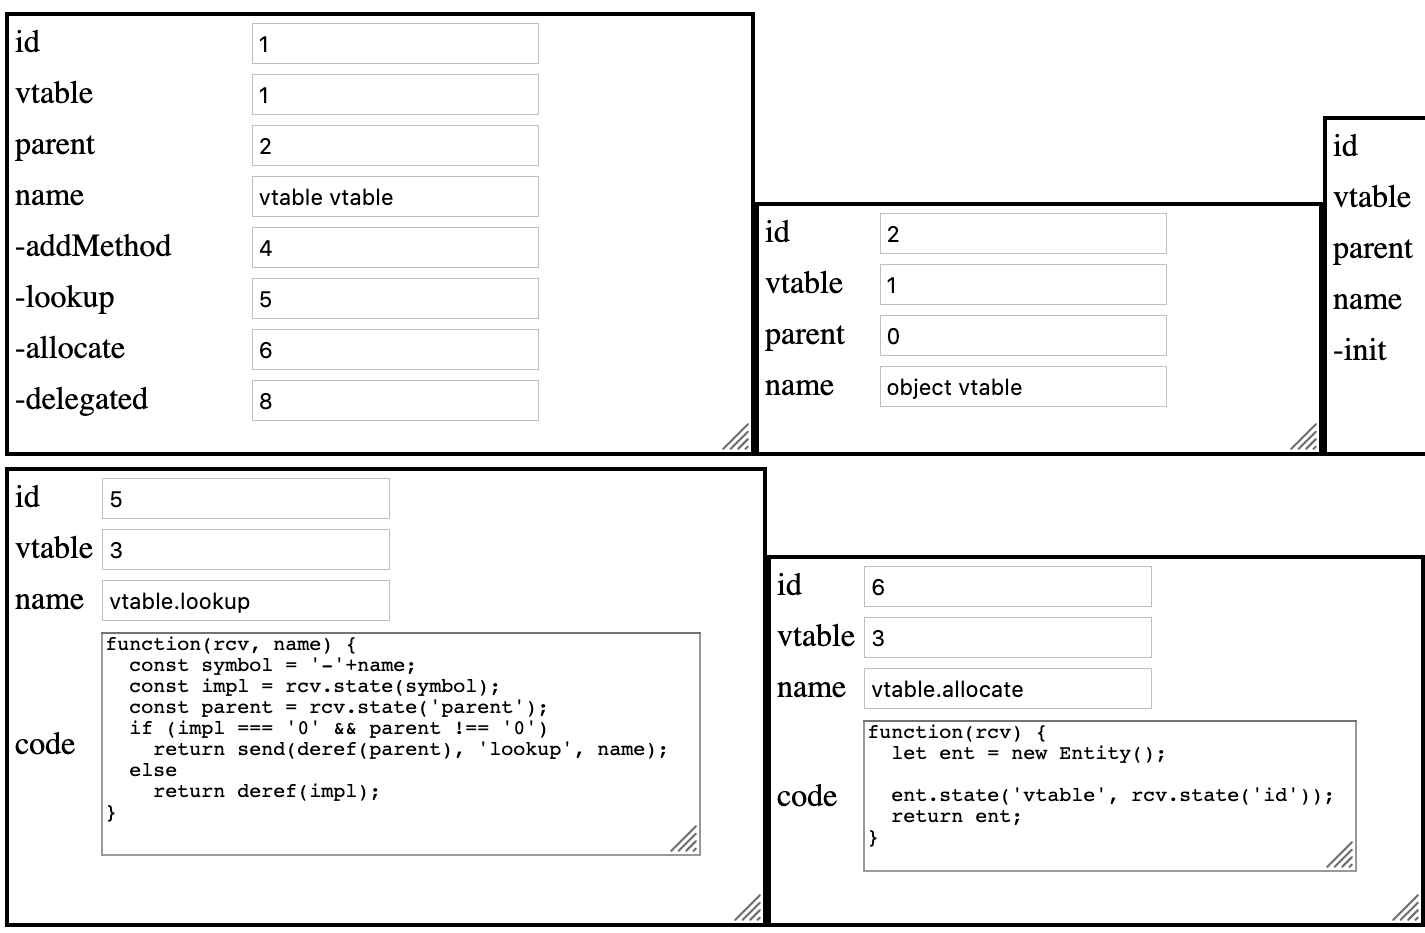
\includegraphics[width=\textwidth]{../orom-html.png}
  \caption{OROM/HTML: Obj-dicts are rendered as resizable tables, which reference
           each other through numerical IDs. \label{fig:orom-html}}
\end{figure}

To emphasise the tendency of OROM objects to be visualised as key-value
mappings, I will refer to them as \emph{obj-dicts}. Figure
\ref{fig:orom-html} shows the OROM/HTML implementation, in which they
take the form of HTML tables.

Here, I was grateful for the browser's management of graphical layout,
resizable text fields, and keeping the DOM tree synchronised with what
one sees. This last property enabled me to make the decision to
\emph{directly} encode much of the system state in the DOM, achieving
basic liveness\footnote{``The thing on the screen is the actual thing''}
for the keys and values of obj-dicts.

For each obj-dict I used a two-column
\texttt{\textless{}table\textgreater{}} within a
\texttt{\textless{}div\textgreater{}}, matching the diagrams, and gave
the rows CSS class names matching the keys for easy lookup. Sending
messages relied on the JavaScript console, but existing values in text
boxes (such as method implementations) could be edited directly. Also
thanks to the browser, I could easily make text boxes and
\texttt{\textless{}div\textgreater{}}s resizable as necessary.

However, the choice of ordinary HTML as a substrate proved rather
two-edged. The browser requires many features to do its job of rendering
complex web pages. And sadly, as its client, I could only make use of
those capabilities which the W3C had decided, at the time of authorship,
were worth the effort exposing in JavaScript. For anything else, the
browser is a black box, and this was very frustrating in the following
case.

\hypertarget{the-radical-concept-of-arrows-that-stay-on-the-shapes}{%
\subsubsection{The Radical Concept of Arrows That Stay On The
Shapes}\label{the-radical-concept-of-arrows-that-stay-on-the-shapes}}

A key aspect of the OROM system is that there is an object \emph{graph}.
That is, obj-dicts can have entries pointing to other obj-dicts, without
restriction to a tree structure. Drawing arrows between things to denote
this is a no-brainer, and I wanted it in my substrate for OROM to match
the diagrams.

A small problem to surmount first: even though I could hijack the
\texttt{\textless{}table\textgreater{}} for its display properties, what
element could I hijack to make arrows between arbitrary points? Luckily,
there was SVG at my disposal, which could be persuaded to display over
the HTML. However, another key feature of my intended substrate was to
be able to rearrange and resize the boxes as desired. So I would also
need to detect changes to the position and size of an element.

Bizarrely, there is no such facility provided for HTML elements. This,
despite the fact the browser \emph{needs} this functionality hence it
must reside \emph{somewhere} inside the black box.

Reluctantly, I stuck with my plan B: each object has a numerical ID and
pointers are just fields containing a number, followed using a
\texttt{deref()} function.

At this point it was starting to look like a mistake not to have done
the whole thing in SVG. I would gain full graphical freedom, though also
lose some benefits of the browser's managing it on my behalf. I already
knew from experience the surprising complexity of a DIY approach to
layout, model-view updates, and interactivity. But such an exercise
would be an opportunity to carefully observe this tedium, and
crystallise some of my intuitions about why it is so consistently
frustrating.

\hypertarget{practicality-vs.-high-aesthetics}{%
\subsection{Practicality vs.~High
Aesthetics}\label{practicality-vs.-high-aesthetics}}

There is the view that insists on provably-correct code written with
strange Unicode symbols, and at the opposite end there is the attitude
of ``get the job done'', high style be damned. Each has its merits, but
for my task I quickly saw the latter route to be most suitable.

My favourite example of this has been the ``encoding'' of obj-dicts as
DOM trees containing particular arrangements of children. In OROM/HTML,
I would gleefully get/set state by calling code like this:

\begin{lstlisting}[language=JavaScript]
Entity.prototype.addState = function(key) {
  let tr = document.createElement('tr');
  tr.setAttribute('class', key);

  let td = document.createElement('td');
  td.setAttribute('class', 'key');
  td.textContent = key;
  tr.appendChild(td);
  ...
\end{lstlisting}

and in OROM/SVG the story is similar. It takes advantage of the powerful
developer tools included in browsers (e.g.~the DOM inspector), and
avoids the need to manually synchronise separate Model and View for such
encoded state. With a little work, it also allowed the system to be
saved and restored --- see Section \ref{persistence}. I consider this as
practical, expedient, ``hijacking'' of these substrates because it
either goes against their intended use (HTML tables for presentation
rather than semantics) or are simply ``odd'' (using certain arrangements
of shapes to ``encode'' machine-readable semantics).

Contrast this with an approach that had to re-synthesise bits of the DOM
whenever something changed. Admittedly this does still happen to a
certain extent, but at least it was minimised where obvious.

Another example of practicality was in the issue of positioning and
sizing. In Section \ref{nut-cracking-with-sledgehammers} I mentioned
that I was able to sidestep some layout work by offloading it to the
user. While building the system I tended to want to draw boxes into
existence, and for that my brain's existing aesthetic algorithms can
decide where they go. There are areas where the machine must be able to
figure this out itself --- I don't want to be constantly bothered by
prompts to place boxes as they are allocated by some running code ---
but for one-offs it is a very convenient way to do a little less
yak-shearing.

\hypertarget{orom-as-svg-trees}{%
\subsection{OROM as SVG trees}\label{orom-as-svg-trees}}

\begin{figure}[h]
  \centering
  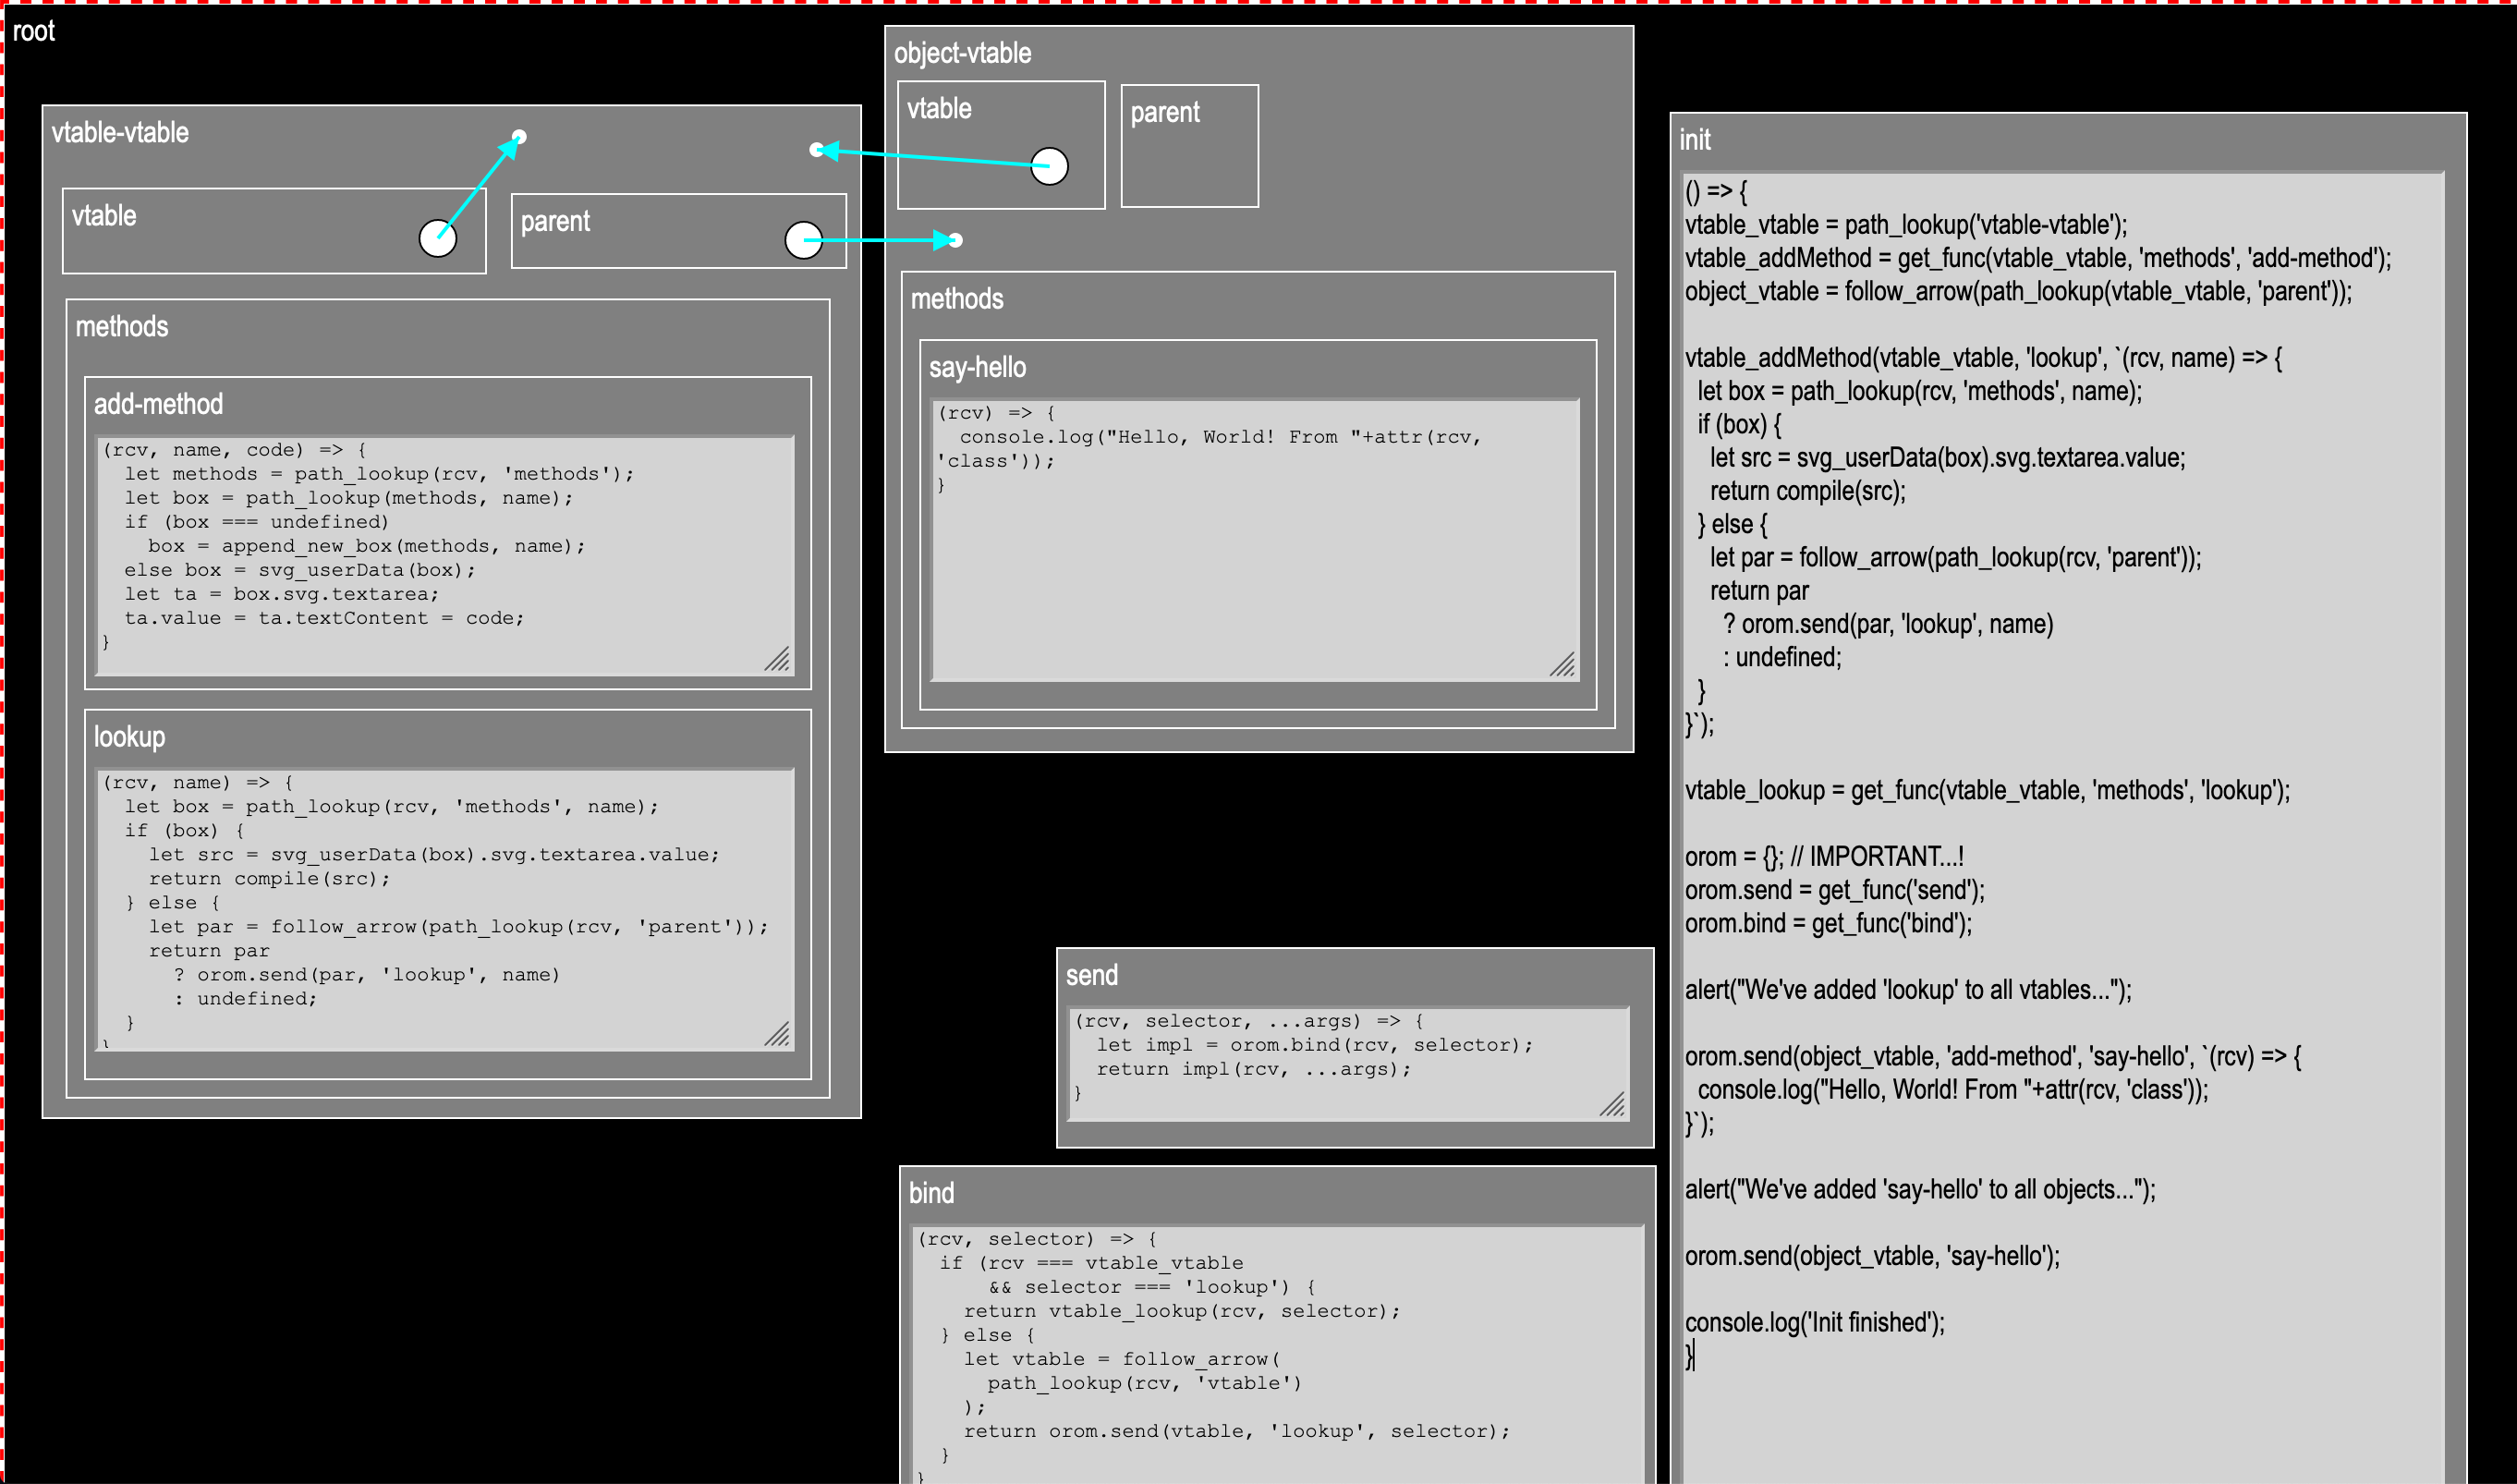
\includegraphics[width=\textwidth]{../orom-svg.png}
  \caption{OROM/SVG: Obj-dicts are moveable and resizable nested boxes,
           referencing each other via real arrows.\label{fig:orom-svg}}
\end{figure}

In this version, shown in Figure \ref{fig:orom-svg}, obj-dicts are
encoded as nested SVG \texttt{\textless{}rect\textgreater{}}s and other
elements, reminiscent of diSessa's Boxer. This was a significant
departure from the table representation, and even though SVG supports
(some) nested HTML via \texttt{\textless{}foreignObject\textgreater{}},
I actually preferred the possibility of multiple levels of nesting.

OROM/SVG more or less realises my desired substrate for implementing
OROM. Needless to say, this version was far more challenging and took
much longer to reach a satisfactory state. However, it is precisely this
drudgery that brings me to a better understanding of this paper's
question: \emph{what has it taken?} I shall discuss this in the form of
broad patterns or themes that stand out to me from my development
experience, hammered home by these OROM projects.

\hypertarget{typical-requirements-of-common-software-and-the-work-we-must-do-to-meet-them}{%
\section{Typical Requirements Of Common Software (and the work we must
do to meet
them)}\label{typical-requirements-of-common-software-and-the-work-we-must-do-to-meet-them}}

The ``common case'' of software present in our daily lives shares
certain properties, such as being graphical and interactive. Such are
expectations that ``end-users'' hold, consigned as they are to merely
\emph{consume} what programmers give them. But if we want to make
``programming'' more like ``using'', such expectations on \emph{use} at
least need to be acknowledged. In this section, I will present these and
other seemingly \emph{inevitable} demands of normal software,
exemplified by OROM/SVG. I will comment how our programming platforms
measure up to the task of helping us meet them, including my chosen
platform of JavaScript and Web technologies.

\hypertarget{retained-mode-vector-graphics}{%
\subsection{Retained-Mode Vector
Graphics}\label{retained-mode-vector-graphics}}

Most software is designed for the subset of people who have a colour
display they can perceive. So right away it is going to require ways to
draw coloured shapes. There are usually libraries for this (though note:
not part of the language), but some only provide \emph{immediate mode}:
commands to instantaneously rasterise pixels to a buffer. This is not
enough for modern software, as we often expect animation, or at least to
see things change as we interact. Most often we wish to see \emph{small
changes} to the \emph{same} shapes, rather than completely different
shapes altogether; the reification that this requires to persist between
frames, is known as \emph{retained mode.}

On this requirement, SVG fits the bill very well. Although it is not
part of the JavaScript language \emph{per se}, it is a standard and
widely supported technology of the Web \emph{platform}. We can observe
that anyone with a browser \emph{in principle} has access to a powerful
vector graphics editor --- just one with no GUI. I will return to this
at the end (Section ??).

The SVG tree keeps the nice properties of the DOM, such as updating the
display when shape parameters are changed. This is well-adapted to
``I/O-bound'' software like mine, where things change only in response
to user input. If I wanted animation, this boils down to a regular
``advance simulation'' signal, and would require setting up some
rendering loop. Alternatively, there is the W3C's chosen ontology of CSS
animations, but see Section \ref{context-appropriate-ontologies}.

\hypertarget{basic-assumptions-about-physical-objects}{%
\subsection{Basic Assumptions About Physical
Objects}\label{basic-assumptions-about-physical-objects}}

In any software making use of vector graphics, there is usually some
level of ``physics'' expected by users. This need not be nearly as
exhaustive as the word ``physics'' might imply, as in e.g.~physics
engines for games; I feel it is important to recognise it for what it is
instead of conceiving physics as an inherently complex thing to be found
only in specialised simulations. For example, pretty much all mobile
apps have what could be called ``phone touch physics'' where menus and
screens slide in and out.

All humans learn a basic set of expectations about the things they see
around them. Some of these, such as ``things fall down'', are not
generally appropriate to software UIs --- perhaps because the screen has
a role in our lives a more of a table work surface rather than a
vertical wall, even if it is vertical in real life.

The level of physics in software tends to not involve force, or mass, or
very much at all, merely position and space; we could call it
``geometric physics''. One thing that all usable software must do, for
example, is not crush many visually complex shapes, such as lines of
text, into the same region, since it becomes unreadable. Such concepts
of ``solid objects do not intersect'' or ``only things at different
layers may overlap'' are basic rules inherited from the real world of
graphical presentation.

I feel the need to point this out, because by default the computer does
not know even the most obvious things about how space works, so we must
laboriously algorithmise this intuitive concept. This is not only true
in the case of 2-dimensional visual domains, but even in the
1-dimensional case of memory allocation. The physics of 1D memory are
something like this:

\begin{itemize}
\tightlist
\item
  This number range 0000-FFFF is like a space, numbers = points
\item
  Every point has at most one owner block
\item
  These blocks are contiguous, finite ranges (i.e.~1D boxes)
\end{itemize}

Hence the boilerplate involved to realise this in any domain with
something resembling space. Far from being a niche topic in games and
graphics, spatial partitioning algorithms and data structures have
surprising relevance to more ordinary software. Both memory allocation
and graphical layout are essential to today's; shame that only one of
those has been recognised as such and entered the runtime of modern
languages.

\hypertarget{translationally-rigid-bodies}{%
\subsubsection{Translationally Rigid
Bodies}\label{translationally-rigid-bodies}}

When you have both a screen and a pointing device (e.g.~touch or mouse),
immediately it becomes worth having ways to move things around in at
least a minimally realistic way. We can debate the appropriateness of
Direct Manipulation (DM) for various situations. But it does make a lot
of sense in simple cases, such moving around subdivisions of space
(e.g.~windows) or elements of a graphical design.

In OROM, the obvious candidate for this is the obj-dicts, plus all
nested boxes in OROM/SVG. If I move the top-level rect, then I expect
its children to move with it. This is simply the translational physics
of rigid bodies: this set of points all move together. Of course, proper
rigid bodies might also rotate and have mass, but this is usually
undesirable for UI elements.

Translational rigidity can be expressed as the points X and Y always
having the same displacement from each other. Or, when one point is
moved, the rest also move by the same delta. This is a problem of
preserving the relationship over time, which was a significant area of
OROM/SVG.

\hypertarget{maintaining-relationships-over-time}{%
\subsection{Maintaining Relationships Over
Time}\label{maintaining-relationships-over-time}}

The model of state-mutation present in most imperative languages is what
I call ``dumb'' state. The language provides an affordance to change any
part of the state to a new value, but nothing else.

What more could there be? Well, in \emph{every} software system there
are certain rules, or ``invariants'' of internal consistency, such as
``translational rigidity'' above. Often, changes to any part of the
system are permissible, but only if connected or dependent parts of the
state change in response.

The job of keeping track of who depends on whom can fall either on the
programmer, or the computer. If the programmer has to do this, they can
only go so far managing and simulating in their head. As systems grow
more complex, it is only natural to try and make the computer more
intelligent to do this work. What I am building up to is that whenever
we (or I) consider constraints, or ``reactive'' programming, or the
``Observer'' pattern as things you only wheel out on special occasions,
we only deceive ourselves into doing the same work less explicitly. It
seems that such ``live state'' should be the expected common case for
software development.

If a platform does not provide a means to causally link and unlink bits
of live state, then this must form part of the standard boilerplate.
Such was the case in OROM/SVG. I implemented the system in an OOP
fashion, and the Observable class is the most widely used. It wraps a
current value and a list of subscribers, notifying them when it changes.

Getting an object to follow the mouse pointer, for example when
dragging, is conceptually very simple: an ``always equal'' relation. In
OROM/SVG founded on live-state, this can be expressed in much the same
way:

\begin{lstlisting}[language=JavaScript, numbers=none]
subscribe(object.position, pointer.position);
\end{lstlisting}

(By default, an Observable A responds to a change from Observable B by
adopting B's new value.)

\hypertarget{nut-cracking-with-sledgehammers}{%
\subsection{Nut-Cracking With
Sledgehammers}\label{nut-cracking-with-sledgehammers}}

Speaking about vector graphics, physics, layout and constraint
maintenance might give the impression of high \emph{conceptual}
complexity at the heart of even simple software. This is not quite true,
which makes it all the worse that there is yet still immense
\emph{incidental} or implementation complexity.

We are conditioned to only think of these in their most general forms.
The vector graphics I use in OROM/SVG are just rects, lines, circles and
text; a fraction of the full capability of SVG. The ``geometric
physics'' I use is dwarfed by fully general 2D or 3D physics engines.
The only layout algorithm I had the patience to implement was a simple
way to expand a list of boxes to fit in a new child at the bottom; the
affordance to place and size boxes \emph{manually} staves off the rest
for the time being! Yet search for material on layout algorithms and it
can seem like Fully General Linear Inequality Solvers like Cassowary are
all there is.

The inevitable requirements I suggest here, do \emph{not} necessitate
Fully General anything. In fact, such representations would make it
\emph{more} cumbersome to express what I wanted in OROM. As the old
wisdom goes, there's no point expressing a simple regex search as an
arbitrary Turing machine; my boxes don't \emph{have} a moment of inertia
or a mass and I don't \emph{need} a linear optimisation solver for my
space management --- for the time being. Under the theme of
domain-appropriate tools, it is worth designing interfaces for
smaller-scale instances of these areas and exploring their capabilities.

\hypertarget{patterns-and-polyfilling}{%
\section{Patterns and Polyfilling}\label{patterns-and-polyfilling}}

The message of the previous section is that existing platforms are often
at the wrong level of abstraction for the requirements of common
software. I recognise that they are reasonably well-adapted to batch
mode file I/O tasks, but that they fail for the \emph{common case} is a
problem. It necessitates largely the same ``boilerplate'' setup per
project just to get basic functionality:

\begin{itemize}
\tightlist
\item
  Here is how I shall describe shapes
\item
  Here is how I make these shapes move together
\item
  Here is how I maintain internal consistency as the user unpredictably
  changes things
\end{itemize}

This burden either falls on the author, or on the wider community to
build and maintain higher-level frameworks, syntax extensions, etc. In
this paper, I refer to this process as ``polyfilling'', with an emphasis
on the DIY, individual level.

It is true, we already have a term for bringing into existence some
software feature that isn't already there: programming. The difference
is that polyfilling is about filling in \emph{boilerplate},
i.e.~functionality \emph{that should have been there in the first place,
but isn't}. This injects some subjectivity and value judgement into the
term. But ultimately, all platforms are designed with certain features
``out of the box'' and leave other features to be implemented ``if
needed''. And when a problem domain ``requires batteries'' yet the tools
available say ``batteries not included'', it is quite reasonable to want
the batteries to be part of the platform.

This section covers the boilerplate I found myself polyfilling in
OROM/SVG.

Is to bring things into the mindset / ontology of the specific software.
For example, wrapping the official Web conventions for event handling in
the Observable infrastructure, or wrapping DOM nodes with ``user data''
objects. The latter case, takes advantage of JavaScript's ability to
simply ``add on'' new fields to objects, even objects of Web APIs, to
``annotate'' the DOM node with a JavaScript helper. Very advantageous to
permit this in JavaScript. In another language like C, such would
require saving the address in a lookup table elsewhere.

\hypertarget{positioning-and-sizing}{%
\subsection{Positioning and Sizing}\label{positioning-and-sizing}}

The simple desire to move and resize boxes with the mouse motivated a
lot of the concepts in Sections
\ref{basic-assumptions-about-physical-objects} and
\ref{maintaining-relationships-over-time}. This problem could be
considered a microcosm of OROM/SVG: what's a natural way I
\emph{conceive} of this behaviour, and could I implement it that way?

It starts with a consideration of translational rigidity. In its most
primitive form, this is a relation between two points. Thus it is
natural to draw a line or ``rod'' between them. It seems that this rod
transmits changes in one of its endpoints directly to the other
endpoint. Since they both feel the same deltas, the displacement vector
between them is preserved (Figure \ref{fig:delta-transmission}).

\begin{figure}[h]
  \centering
  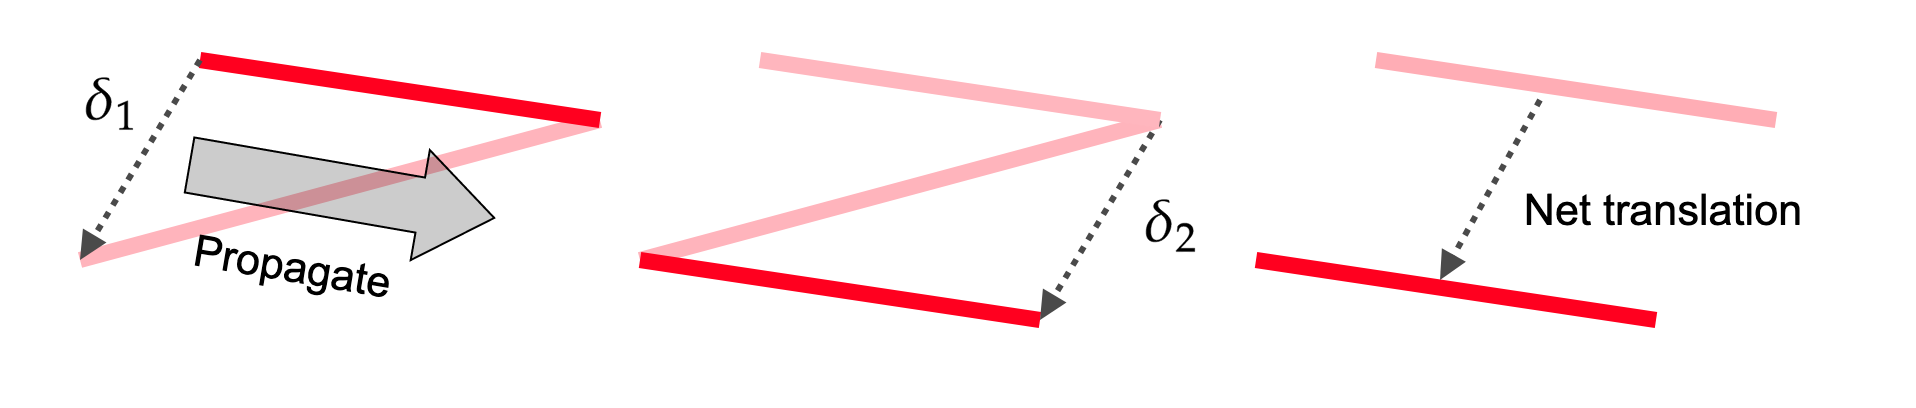
\includegraphics[width=\textwidth]{../delta-transmission.png}
  \caption{Fully rigid rods transmit changes in one end to the other end. \label{fig:delta-transmission}}
\end{figure}

I like to see what I'm doing, so I wanted these rods to be visible and
thus somehow \emph{present in the SVG}. This was not hard; in SVG I draw
a \texttt{\textless{}line\textgreater{}}, though the background
machinery of the Rod class does all the work. There is also a Point
class that is used wherever manipulable points (SVG circles) are
intended.

Resizing of boxes could be achieved through rods that stay horizontal or
vertical. In the language of ``small differences'' spoken by the
live-state infrastructure, this is expressed as a rod ``transmitting
deltas'' in the vertical and horizontal, ``absorbing'' the other
component into itself (Figure \ref{fig:rods}). Mirroring a DOM rect to
these rods is as simple as subscribing its width and height to
horizontal and vertical rods' \texttt{length} Observables. This way,
boxes can be resized from whatever corner is convenient.

\begin{figure}[h]
  \centering
  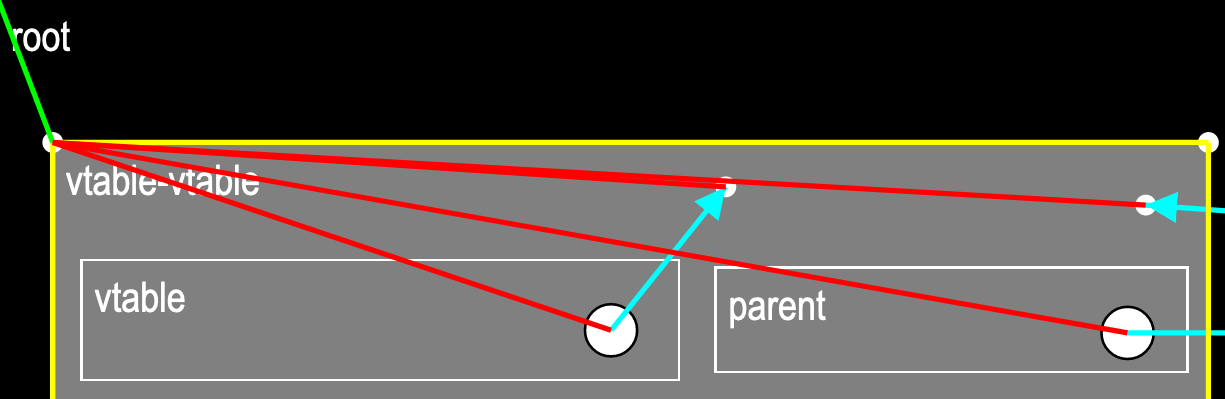
\includegraphics[width=0.75\textwidth]{../rods.png}
  \caption{The yellow rods on the box border are ``half-rigid'': they transmit horizontal or vertical changes, but not both. The green rod in the top-left absorbs all changes from an endpoint into itself, visualising the displacement vector of the child box from its parent. The remaining red rods are fully rigid. A line of CSS can show this ``scaffolding'' which is normally hidden for users. \label{fig:rods}}
\end{figure}

Unfortunately, with these rods came possibly the most frustrating
technical challenges of the entire system. Initially I hoped to move
boxes as rigid bodies by temporarily making their border rods rigid.
However, the four border rods form a cyclic graph, as rods are not
directed. This, coupled with the unintended depth-first semantics of
Observable notification (a result of JavaScript function calls in a
loop), led to duplicate deltas applied twice and other nightmares. This
is the tip of an entire research iceberg stretching from Functional
Reactive Programming to internet routing and distributed algorithms.

I did manage to surmount this through kludging and compromise. But I do
not know whether these problems are merely a consequence of some design
decision I could change to escape it, or if they are intrinsic to my
(modest) UI goal.

\hypertarget{visible-coordinate-systems}{%
\subsection{Visible Coordinate
Systems}\label{visible-coordinate-systems}}

Rigidity in a flat world of sibling shapes is somewhat straightforward.
However, rigidity in the SVG world is more involved.

First of all, SVG shapes (e.g.~\texttt{\textless{}rect\textgreater{}})
are strictly \emph{leaf} nodes of the DOM. So if I wish to nest boxes
within boxes, the visible box \texttt{\textless{}rect\textgreater{}}
must be a mere \emph{accessory} to the nestable element, in my case a
\texttt{\textless{}g\textgreater{}} (group). This means that instead of
resizing the \texttt{x}, \texttt{y}, \texttt{width}, \texttt{height}
attributes of the \texttt{\textless{}rect\textgreater{}}, only its
\texttt{width} and \texttt{height} change, along with the
\texttt{transform} attribute of its \emph{parent}
\texttt{\textless{}g\textgreater{}}. This was not too bad; just
subscribe this attribute, instead of the
\texttt{\textless{}rect\textgreater{}} position, to the top-left Point
handle.

All child elements of a node transform with it, so already SVG has baked
in a basic facility for translational rigidity. This is only available
as a tree hierarchy, but it is still useful. However, it conflicts with
my early decision to have Point objects all share the global co-ordinate
system (this was to ensure that simple relations, such as a point
following the mouse pointer, are not infuriating to express.) Still, it
was necessary in the case of certain elements --- especially those which
must transcend the tree structure altogether, like arrows between boxes
--- to bite this bullet, one way or another.

\begin{quote}
Maybe mention that this is caused by the mismatch between the substrate
and the programming system (substrate is tree, but programming is
graphs)?
\end{quote}

Again, I return to how we tend to work things out in the freedom of
paper. Co-ordinate systems, here merely positionally displaced, have
their origins here and there and have vectors between them. The rods
thus far let me visually express relations between global Points; now
was a question of expressing one global Point as a displacement from
another (the \texttt{\textless{}g\textgreater{}} transform). New rod
Observables \texttt{p2\_from\_p1} and \texttt{p1\_from\_p2} do the
vector subtraction, which can then be propagated as local co-ordinates
to children. It is nicer to express the relation (as well as see it!)
this way (Figure \ref{fig:rods}).

\hypertarget{context-appropriate-ontologies}{%
\subsection{Context-appropriate
ontologies}\label{context-appropriate-ontologies}}

Each API has its own conventions, including a way of naming and
structuring expressions --- an ontology. The One-Size-Fits-Allapproach
is exemplified in such interfaces. For example, in SVG we express a
rectangle by
\texttt{\textless{}rect x="10" y="10" width="600" height="400"\textgreater{}}.
The SVG specification \emph{defines} to the user that a rect \emph{is} a
top-left corner, a width, and a height --- and that's it. However, this
SVG-approved parametrisation of a rectangle is far from the only
one\href{https://www.shift-society.org/salon/papers/2018/critiques/critique-semprola.pdf}{1},
and thus is, unsurprisingly, ill-fitted to some contexts.

For example, I find it natural to resize boxes by dragging any of their
four corners, so I wanted this in OROM/SVG. In this context, a
``rectangle'' is \emph{seen as} four points: top-left, top-right,
bottom-left, bottom-right. Obviously this is not a \emph{minimal}
description, since given e.g.~the top-left and bottom-right, the other
two points can be inferred. But one way or another, to be able to drag
any of them, all four points must be present at \emph{some} level. This
alternative ontology was polyfilled in the form of a ``rect controls''
class that can be attached manually to any SVG
\texttt{\textless{}rect\textgreater{}}. The \texttt{x} and \texttt{y}
are subscribed to the top-left Point\footnote{In the usual case where
  the \texttt{\textless{}rect\textgreater{}} is part of a box, the
  top-left instead controls the parent
  \texttt{\textless{}g\textgreater{}}'s \texttt{transform} --- but the
  idea is the same.}; \texttt{width} and \texttt{height} are subscribed
to Rod lengths.

Another example is to be found in the DOM's event listener model.
Conceptually, many ``events'' are in fact changes to the state of some
physical (or conceptual) device. And both keyboard keys and mouse
buttons, for example, have two states --- pressed, not pressed --- which
ought to make them \emph{interchangeable} to this extent. This is the
logic behind ``key mapping''\footnote{For example, the player can
  re-assign the action ``shoot'' from its default mouse button to a
  keyboard key, or another action from keyboard to mouse, as it suits
  them.} in PC games. But the official ontology of the Web makes it
nontrivial to do this.

To start with, the situation is modelled not as a time-varying value
changing, but instead as a sort of Cartesian product of event listeners.
Rather than, say, a piece of live-state for the left mouse button (LMB),
we get \texttt{onmousedown} and \texttt{onmouseup}. Thankfully we do not
have \texttt{onAdown}/\texttt{onAup}, \texttt{onBdown/onBup}, \ldots{}
all the way to \texttt{onZdown}/\texttt{onZup}, but only
\texttt{onkeydown}/\texttt{onkeyup}. Yet this is just one of the many
possible ways to slice this 3-dimensional\footnote{Device (mouse,
  keyboard), sub-device (button, key), state (up, down)} space.

In OROM/SVG I did not quite want to re-map keys, but I did often want to
have things follow the mouse when dragged. In order to do this, I
reified the mouse pointer and its position, letting me write
\texttt{subscribe(point.position,\ pointer.position)}. The Point has an
\texttt{is-considering-me?} Observable wrapping
\texttt{onmouseover}/\texttt{onmouseout}, and the LMB is reified into
\texttt{left\_mouse\_button\_is\_down} to be explicit. The
aforementioned subscription is set up whenever
\texttt{is-considering-me?} and \texttt{left\_mouse\_button\_is\_down}
become true, and torn down otherwise. I tended to think of this in the
form ``subscribe to pointer \emph{only when} pointer is-considering-me
\emph{and} LMB is down'', but I could live with this as a future
polyfill in JavaScript.

The way these things are connected to the browser's event listeners
could be called ``device drivers''. This approach is described in more
detail in \href{https://prog21.dadgum.com/66.html}{13}. It amounts to
translating information from the ``unchangeable'' Web platform into the
worldview of my substrate, as early as possible:

\begin{lstlisting}
svg.onmousedown = e =>
  if (e.button === 0) change(left_mouse_button_is_down, true);

svg.onmouseup = e =>
  if (e.button === 0) change(left_mouse_button_is_down, false);

svg.onmousemove = e => {
  let r = svg.getBoundingClientRect();
  let pos = vsub([e.clientX, e.clientY], [r.left, r.top]);
  change(pointer.position, pos);
};
\end{lstlisting}

It takes some frustration and experience to get used to the idea that
you have a right to polyfill in alternative representations. Before I
came to this conclusion, I used to twist my head around translating my
intention into the \texttt{x,y,width,height} parameters, and
un-translating when reading back the code I had produced. Once you get
used to having to adapt your mental imagery to a single way of doing
things (i.e.~learning to code), it makes sense to simply expect to see
more of it --- especially when you know you are new, surrounded by
veterans who see no problem, and so on. Nowadays, I take the position
that these are simply \emph{widespread} failings of our way of doing
things, instead of \emph{our} failure to adapt to the way software is.

What would it look like to support multiple ontologies? There are the
two answers: anticipate the possibilities ahead of time, or support
users adding their own. It is unclear if we can do better on the latter
than simply ``support polyfilling''. As for the former: in general,
anticipating the diversity of ways someone might look at the world is
doomed to fail. But in the case of fairly \emph{formalised} concepts
such as geometrical shapes or mathematics, I could suggest that simple
\emph{under-specification} is the root of the problem in SVG. Instead of
explaining in English that ``\texttt{x} and \texttt{y} are the
co-ordinates of the top left-hand corner\ldots{}'', it might be better
to make these relations machine-readable or \emph{embodied} in the API.
For the rect this might look like:

\noindent A \texttt{rect} is\ldots{}

\begin{itemize}
\tightlist
\item
  a \texttt{polygon} (defined elsewhere)
\item
  defined by 4 \emph{degrees of freedom} \texttt{x\ y\ width\ height}
  (internal representation)
\item
  where there are 4 \emph{vertices}, all \texttt{point}s

  \begin{itemize}
  \tightlist
  \item
    \texttt{{[}x,y{]}} ``top-left''
  \item
    \texttt{{[}x+width,y{]}} ``top-right''
  \item
    \texttt{{[}x,y+height{]}} ``bot-left''
  \item
    \texttt{{[}x+width,y+height{]}} ``bot-right''
  \end{itemize}
\end{itemize}

The hope is that if we then specify enough information --- say, the
bot-left and top-right --- then the runtime has all it needs to derive
its internal 4 degrees of freedom.

In a crude sense, I have successfully anticipated the most obvious
ontologies of a rectangle here. However, I missed out the ``centre plus
half-width and half-height'' formulation, among others. Is this a futile
effort even for precise mathematical knowledge structures, or could
enough formalisation of Euclidean geometry in the Web platform put an
end to this sort of polyfilling?\footnote{This relates to my intuition
  that type systems and other auto-reasoning tools are trapped in a
  doomed quest for ``closed-form'' AI, representable as a
  \LaTeX formula.}

\hypertarget{extensional-functions}{%
\subsection{Extensional Functions}\label{extensional-functions}}

Time and time again we come across the same pattern of partitioning
system state: trees or graphs of dictonaries, a.k.a. Maps, a.k.a.
associative arrays. I am talking about filesystem paths
\texttt{/path/to/some/file}, Python / Java modules
\texttt{com.example.pkg.subpkg}, JavaScript objects
\texttt{window.my\_obj.component}. The common case is an association of
a textual (string) name, to an arbitrary value. I find it useful to see
this as a mathematical ``function'' defined \emph{extensionally} by
listing its input/output mappings --- this opposed to an
\emph{intensional} definition such as \(x \mapsto 2x+3\), or a computer
program.

Extensional functions are perhaps the most basic form of Knowledge
Representation, and match natural language very well. ``The bicycle's
wheels' spokes are silver'' straightforwardly translates to a function
equation
\texttt{root\ (bicycle)\ (wheels)\ (spokes)\ (colour)\ =\ root\ (silver)}.
That is, whatever object is the output of \texttt{silver} in the
top-level \texttt{root} function, the output of \texttt{colour} (in the
function on the left) points to the same object. The ability to
partition a system in this way enables what
\href{https://github.com/amb26/papers/blob/master/ppig-2016a/ppig2016a.pdf}{2}
calls a ``natural co-ordinate system'' for a piece of software, crucial
for understanding and adaptability by others (so long as it is
externalised).

It seems that this way of expressing the ``parts'' of a system is an
inevitable requirement of any programming substrate. Some languages,
such as C, do have static, \emph{compile-time} associative arrays
(\texttt{struct}s). In my experience this is usually not enough, and
it's necessary to bring in a library or clutter the code with a
home-grown approximation to dynamic ones. Some parts of the OROM
authors' C code were confusing until I realised they were just the guts
of a basic associative-array implementation; when I switched to
JavaScript, these lines vanished.

Perhaps another strength of JavaScript is its low \emph{concrete syntax
cost} for \emph{instances} or \emph{literals} of associative arrays.
Writing or reading

\begin{lstlisting}
a = {
  b1: { c1: z, c2: y },
  b2: { c3: x, c4: w }
};
\end{lstlisting}

is more WYSIWYG\footnote{What You See Is What You Get} than the
imperative-style

\begin{lstlisting}
a = new Map();
a.set('b1', new Map());
a.get('b1').set('c1', z);
a.get('b1').set('c2', y);
a.set('b2', new Map());
a.get('b2').set('c3', x);
a.get('b2').set('c4', w);
\end{lstlisting}

The latter is unfortunately still required in JavaScript for extensional
functions with \emph{non-string} inputs.

The decision to switch from the flat tabular representation in OROM/HTML
to the nestable, Boxer-like structure in OROM/SVG permitted extensional
(tree) functions in its substrate. True, I could always encode these in
flat tables by having them reference each other. But this is like the
second listing above: hard to follow. In the case of distinguishing
between ordinary state mappings and the ``method dictionary'' of
vtables, I actually stored method mappings with a ``-'' character to
avoid doing this (Figure \ref{fig:method-hyphens}). In OROM/SVG, I can
directly express the model I was thinking of (Figure
\ref{fig:method-boxes}).

\begin{figure}[h]
  \centering
  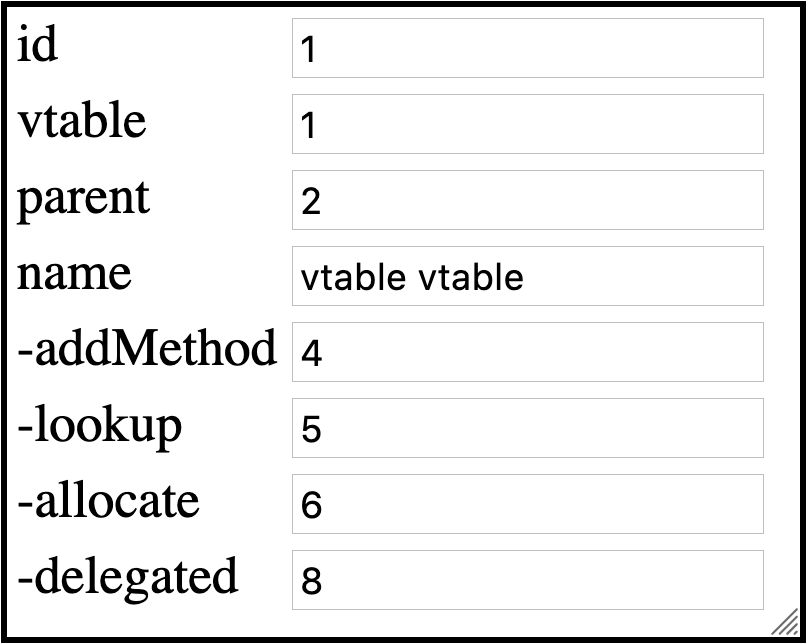
\includegraphics[width=0.5\textwidth]{../method-hyphens.png}
  \caption{OROM/HTML: use of hyphenated \texttt{-lookup} to signify a \emph{method} called
           \texttt{lookup} instead of a property like \texttt{vtable}. \label{fig:method-hyphens}}
\end{figure}

\begin{figure}[h]
  \centering
  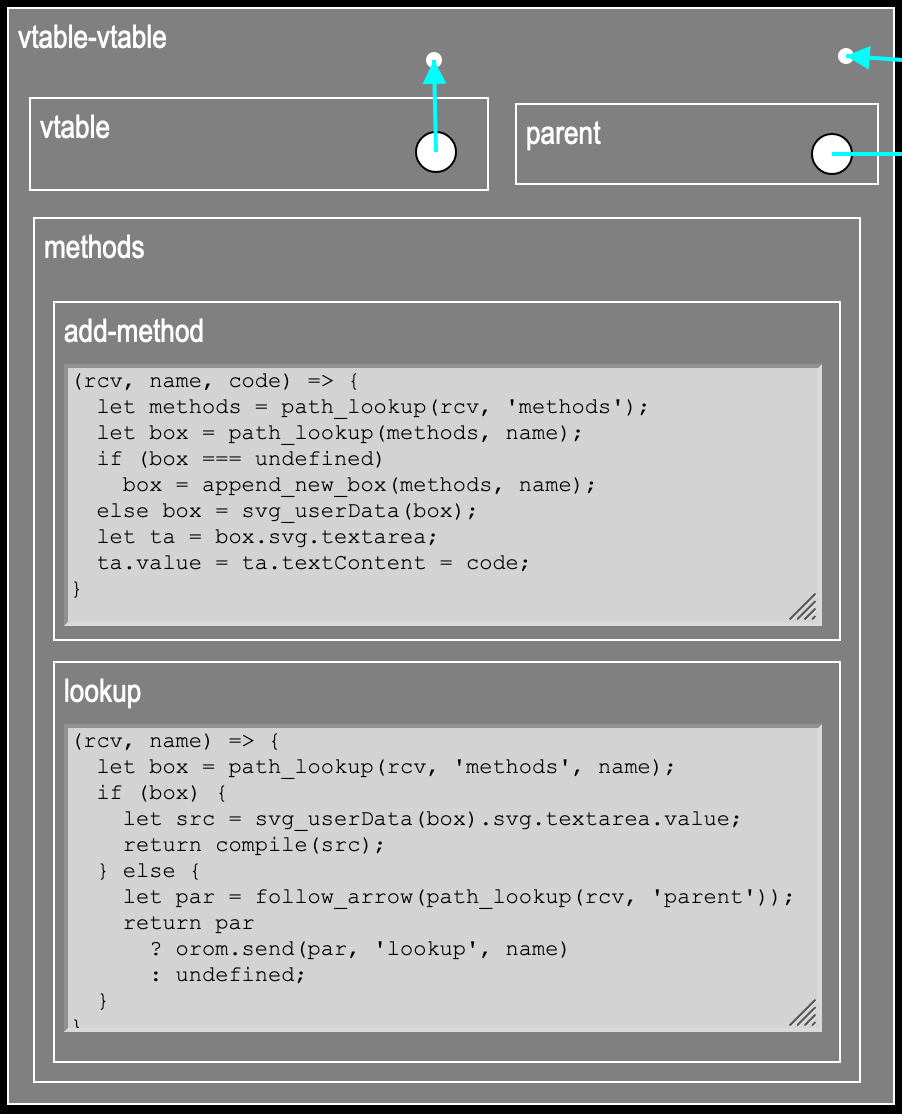
\includegraphics[width=0.5\textwidth]{../method-boxes.png}
  \caption{OROM/SVG: the \texttt{vtable} box has a \texttt{methods} box, and that's where the method boxes go. \label{fig:method-boxes}}
\end{figure}

\hypertarget{persistence}{%
\subsection{Persistence}\label{persistence}}

This refers to exposing structured program state to the user. This data
can then be saved and used to restore the system at a later date, but it
can also be tweaked with corresponding changes reflected in the system.

Persistence was absolutely necessary to continue OROM/SVG development,
past a certain point. This is because, upon discovering a bug and fixing
it in the source code, the web page must be refreshed and started anew.
In the beginning, when verifying that box drawing with the mouse is
working correctly, this is not much of a problem: upon refresh, the
blank initial state is restored and I could draw again. But as the
substrate matured, and I began to implement parts of the target system
(OROM) --- the cycle of finding a bug, tearing down the system,
refreshing and losing work, and manually building it up again, proved
frustrating. Because the system could only be patched externally and
restarted, there needed to be some way to persist changes that
\emph{weren't} part of the code, but the DOM instead.

Normally, this can be as simple as autosave to the filesystem. But the
Web platform is very wary of this\footnote{As anyone who learns WebGL
  can attest to, when they discover they must run a local Web server to
  provide image files for textures since any filesystem requests will be
  rejected for security.}, so the solution I turned to was manually
copying the markup in the browser's inspector (Figure
\ref{fig:html-inspector}).

\begin{figure}[h]
  \centering
  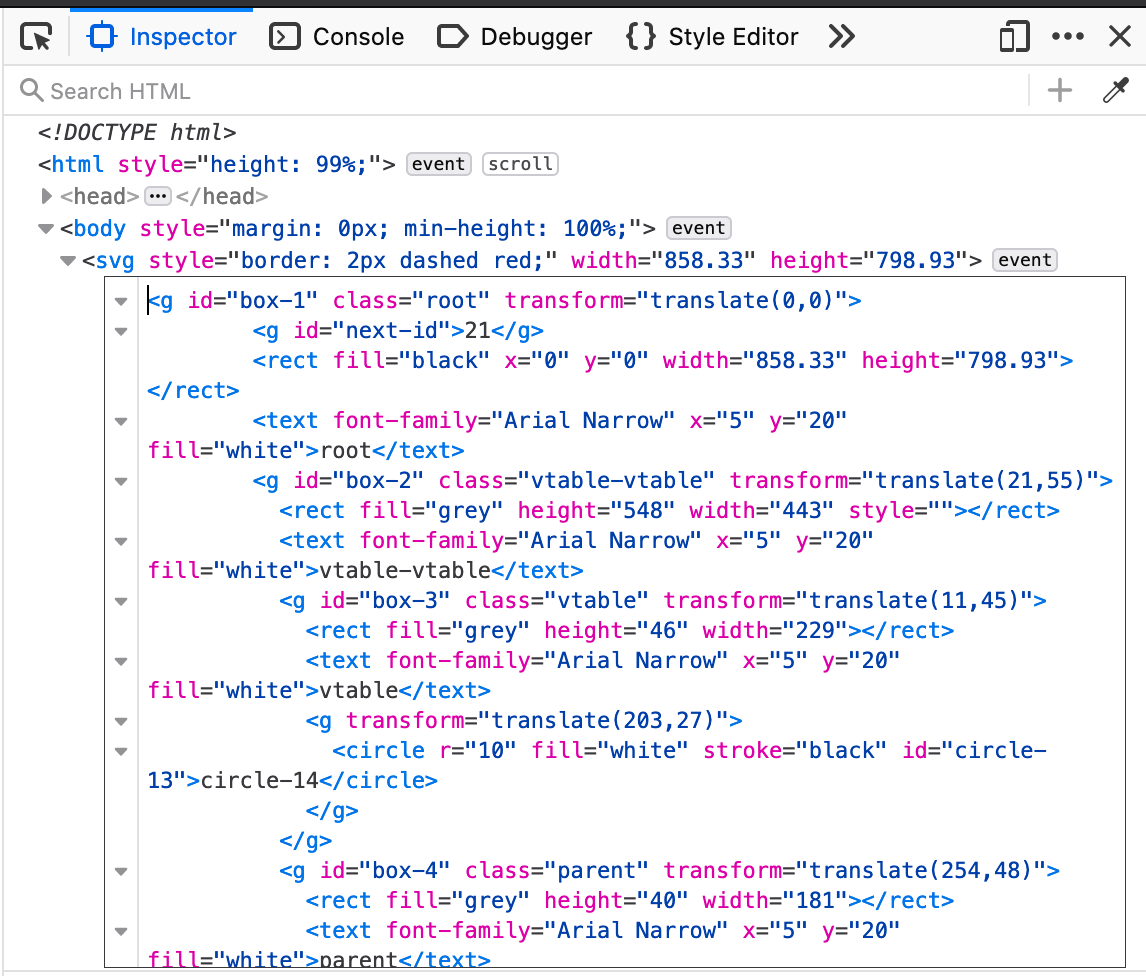
\includegraphics[width=0.8\textwidth]{../html-inspector.png}
  \caption{To save the state of the system, the SVG group corresponding to the \texttt{root} box is copied and pasted inside the HTML file's \texttt{\textless{}svg\textgreater{}} element.\label{fig:html-inspector}}
\end{figure}

This required a slight change towards an architecture where the all the
data required to reconstruct the system's current state is contained in
the inspector HTML (plus the OROM/SVG JavaScript source code.) Where
previously ``boxes'' were created first as invisible JavaScript objects
responsible for some SVG, now it was the other way round. When a rect is
clicked, the system must look at some SVG and interpret it ``on demand''
as a box (lazily initialising its helper object if so).

Persistence seems to be a weaker cousin of \textbf{externalisability},
defined in \href{antranig}{1}. As it stands, the system does not quite
qualify as externalisable. When making changes to the HTML in the
element inspector, the system's behaviour \emph{should} adjust to match,
but this is not currently guaranteed in all cases.

\hypertarget{the-orom-system-as-a-part-of-the-solution}{%
\section{The OROM system as a part of the
solution}\label{the-orom-system-as-a-part-of-the-solution}}

The OROM system was designed with a goal of eliminating the
``artificial'' distinction between implementation language and end-user
language, by means of a mostly self-defining, or ``meta-circular''
object model. This general way of working on a piece of software ``by
means of itself'' is easy to agree with, even if OOP is not to
everyone's taste. It is an open question whether OROM's approach could
be applied to other programming styles.

The allure of meta-circularity here is not merely in being ``cool'', but
that it paves the way to end-user empowerment. This is somewhat
misleading because in OROM, these ``end-users'' are actually
programmers. However, its purpose is to free a programmer's dependence
on some distant and busy language designer, and it seems plausible that
this is a stepping stone on the way to enabling programmers to
\emph{create} a piece of software which non-programmers do not depend on
them for.

I emphasise that this is the \emph{allure} of OROM. However, there are
some significant practical issues that must be overcome or clarified
first.

\hypertarget{minimal-descriptions}{%
\subsection{Minimal descriptions}\label{minimal-descriptions}}

The OROM paper was part of the STEPS project of Alan Kay's
VPRI\footnote{Viewpoints Research Institute}. This project argued that
the immense level of ``accidental complexity'' present in software
implementation could be reduced, and Kay himself dreams of an end result
analogous to a ``Maxwell's Equations'' of software. That is: the
behaviour of electromagnetic fields can be represented in four short
equations that fit ``on a T-shirt''. A self-hosted LISP interpreter fits
on a page. Could we aim at a similar ``fundamental description of
software'' that fits on something less than millions of lines of code?

This argument as stated suffers by glossing over an important fact.
Maxwell's equations certainly do fit onto a T-shirt, but most people
will not be able to explain what they mean. What typically amounts to
years of study is compressed into those mathematical symbols, and the
learning material involved most certainly does \emph{not} fit on a
T-shirt. The obvious \emph{reductio ad absurdudum} is where we
encapsulate these equations under a single symbol, M. M is defined as
``Maxwell's Equations are true''. Ta-da --- this fits on a coin, but
good luck doing anything with it.\footnote{In fact, this is almost
  achieved by the formalism of Geometric Calculus, which reduces them to
  only one equation.}

I say this not to dismiss the argument, but to highlight the actually
hard part of getting a ``concise description'' of some system; defining
complexity away into a symbol helps us no more than naming the solution
to an equation ``x''. There is a connection with data compression: even
if the data successfully compressed into a smaller file, the size of the
compression \emph{program} should be added as well. What matters is to
reduce the \emph{combined} size of notation and platform.

We have a word ``re-factoring'', but what about the ``factoring'' in the
first place? The previous discussion of ``ontologies''

Further, there is perhaps a risk of optimising for \emph{formal} rather
than \emph{practical} minimality (e.g.~the Turing machine). OROM's
``minimality'' does not necessarily translate into ``simplicity''; it
suffers from the same \emph{cognitive} complexity, or need for study, as
Maxwell's Equations. I cannot stress the amount of effort I have put in
to wrap my head around the self-referential ``vtable vtable'' and the
task of self-implementation. An overall better system might be one which
is easier to pick up or understand, even if the number of formal objects
is not as minimal.

\hypertarget{self-implementation}{%
\subsection{Self-implementation}\label{self-implementation}}

This is also cool, but hard.

Other themes e.g.~homoiconicity of code and data

``Taming'' SVG - ability to use SVG in a vaguely sane way (vector
graphics editor)

Similarly for e.g.~3D OpenGL, Web Audio, sockets \ldots{}

\hypertarget{tensions-between-philosophies}{%
\subsection{Tensions between
philosophies}\label{tensions-between-philosophies}}

\hypertarget{stable-or-emergent-antranig-against-oop-dispatch}{%
\subsubsection{Stable or emergent? (Antranig against OOP
dispatch)}\label{stable-or-emergent-antranig-against-oop-dispatch}}

\hypertarget{turing-complete-antranig-against-this}{%
\subsubsection{Turing-complete? (Antranig against
this)}\label{turing-complete-antranig-against-this}}

\hypertarget{messaging-vs-read-write}{%
\subsubsection{Messaging vs Read-Write?}\label{messaging-vs-read-write}}

\hypertarget{conclusion-and-future-work}{%
\section{Conclusion and future work}\label{conclusion-and-future-work}}

Conclusion: what I have that Maxwell's E doesn't.
